\section{Dijkstrův algoritmus}\label{sec:dijkstra}

Již jsme si ukázali, že v \emph{neohodnoceném grafu} $G=(V,E)$ umíme relativně jednoduše najít délku nejkratší cesty do libovolného vrcholu z nějakého výchozího vrcholu $v_0\in V$. Obvykle však hrany nemusí mít stejnou váhu (cenu). Cesty (vrcholy) mezi městy (hrany) mohou být v různém stavu a některé jsou tak lepší než jiné.
\importantbox{Zde ji narážíme na problém, neboť obecně platí, že když nalezneme vrchol přes dvojici různých hran, nemusí být nalezené cesty stejně dlouhé. Na obrázku \ref{fig:ohod_graf} si lze všimnout, že cesta $(v_0,v_1,v_2)$ je kratší než $(v_0,v_2)$, přestože má více hran.}
\begin{figure}[h]
    \centering
    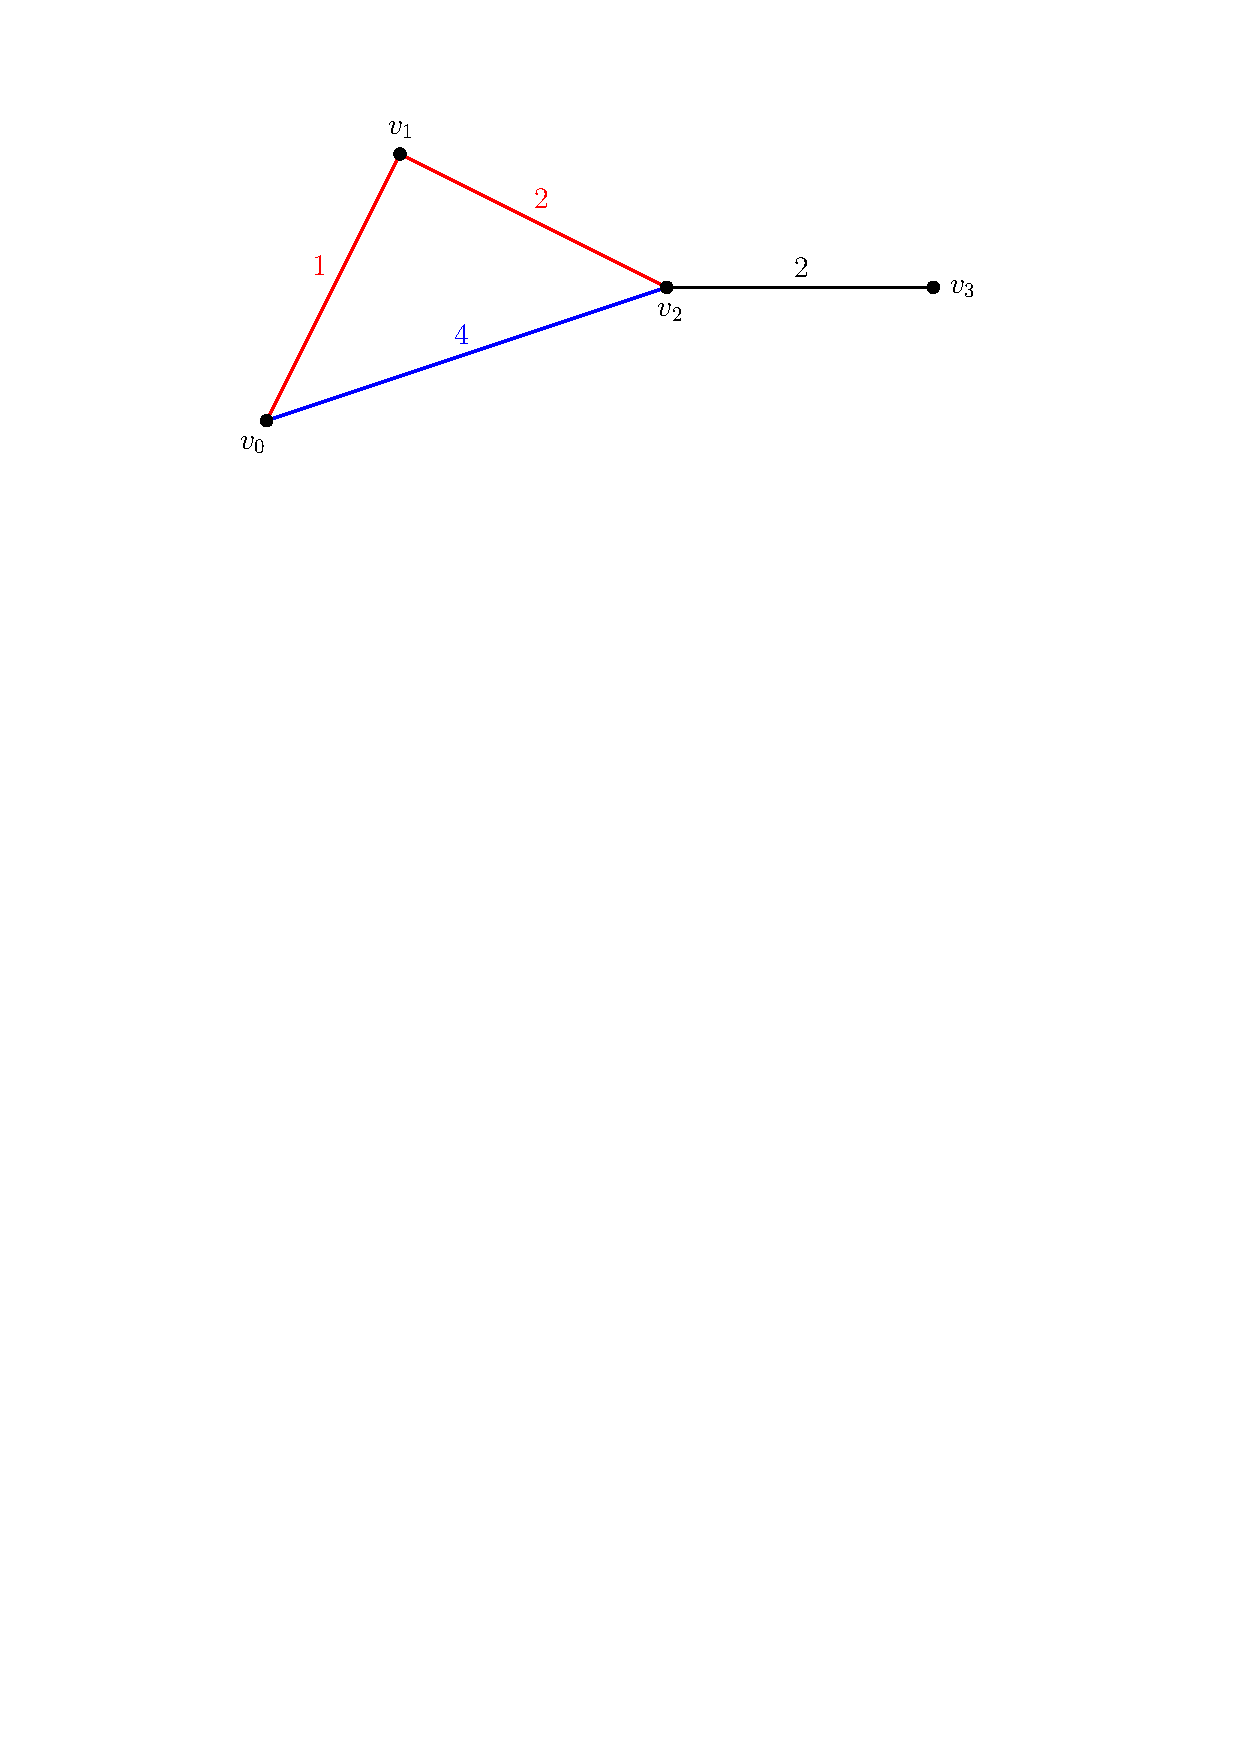
\includegraphics[scale=\graphimgsize]{components/images/ch01_ohod_graf.pdf}
    \caption{Příklad ohodnoceného grafu.}
    \label{fig:ohod_graf}
\end{figure}
Nabízí se varianta převést ohodnocený graf na neohodnocený tak, že rozdělíme hranu na takový počet hran, kolik činí její původní váha.